In 2009, researchers placed a dead salmon in an MRI scanner, showed it photographs of humans in social situations, and ostensibly asked it to judge their emotions \citep{bennett2009neural}. Standard analysis pipelines commonly used at the time surprisingly returned brain voxels as significantly predictive of emotional situations. The error arose from a failure to correct for multiple comparisons within the statistical analysis pipeline. The “dead salmon” demonstration of false positives contributed to a larger reckoning in the field of neuroscience. For instance, an influential study showed that different research groups obtained different results even when analyzing the same dataset and the same research question~\citep{botvinik2020variability}. 
Subsequent work identified several sources of \textit{statistical fragility}. Widely used statistical procedures embedded in standard analysis pipelines were shown to inflate false-positive rates~\citep{eklund2016cluster}, an effect worsened by non-independent analyses producing spuriously large brain–behavior correlations~\citep{vul2009voodoo}. Also, early neuroimaging research was constrained by small samples and limited data availability~\citep{button2013power,marek2022reproducible}, exacerbating overfitting and spurious associations. Moreover, fMRI had been criticized for offering predictive explanations, rather than functional ones, resulting in little clinical relevance~\citep{lyon2017dead}. Finally, reverse inference emerged as a central interpretative problem, given that individual neural systems are not uniquely associated with specific cognitive functions~\citep{poldrack2006can,duncan2000common}. 

AI interpretability now faces its own \textit{dead salmon} issues, similarly begging for a larger reevaluation of its statistical foundations. A growing body of work has shown that many influential methods, including feature attribution \citep{adebayo2018sanity}, probing classifiers \citep{ravichander-etal-2021-probing}, sparse autoencoders \citep{heap2025sparseautoencodersinterpretrandomly}, circuit discoveries \citep{melouxeverything}, and causal abstractions~\citep{sutter2025nonlinearrepresentationdilemmacausal}, can yield plausible-looking explanations even when applied to \textbf{random neural networks}. In Figure~\ref{fig:illus}, we report a minimum dead salmon artifact from analyzing activations of a fully randomized BERT model in a sentiment analysis task where both correlation analysis and probing find highly significant \textit{explanations}. Such striking failure modes are particularly troubling as modern AI systems are increasingly deployed in high-stakes domains where AI interpretability should be essential for transparency, accountability, and error diagnosis~\citep{mehrabi2021survey,barnes2024navigating,ramachandram2025transparentaicaseinterpretability}. 
Interpretability methods have the potential surface critical failure modes~\citep{kim2017interpretable,zech2018variable,caruana2015intelligible,meng2022locating,monea2024glitchmatrixlocatingdetecting,nguyen2025deploying} and offer levers for mitigating bias and systematic errors \citep{arrieta2019explainableartificialintelligencexai,kristofik2025bias,lepori-etal-2025-racing}. 

Yet, despite frequent analogies to mature sciences like \textit{neuroscience}~\citep{barrett2019analyzing}, \textit{biology}~\citep{lindsey2025biology}, or \textit{physics} \citep{AL2023-cfg,AllenZhu-icml2024-tutorial} of neural networks, the practice of AI interpretability remains in its early foundational stages. Striking dead-salmon artifacts are accompanied by a general statistical fragility: small perturbations to inputs \citep{Ghorbani_Abid_Zou_2019,Kindermans2019,pmlr-v260-zhang25a} or changes in random initialization \citep{adebayo2018sanity,zafar-etal-2021-lack} can radically change explanations. Explanations often fail to generalize to new settings and input distributions \citep{hoelscherobermaier2023detectingeditfailureslarge}. Also, multiple incompatible explanations can be \textit{discovered} for the same behavior~\citep{melouxeverything,NEURIPS2019_bb836c01}. While the dead salmon study demonstrated a simple statistical oversight correctable through multiple comparison adjustments, AI interpretability's difficulties stem from more fundamental issues. In particular, we argue that, for common interpretability queries, computational traces do not uniquely determine explanations.

\begin{wrapfigure}{tr}{0.50\textwidth}
    \centering
    \vspace{-1em}
    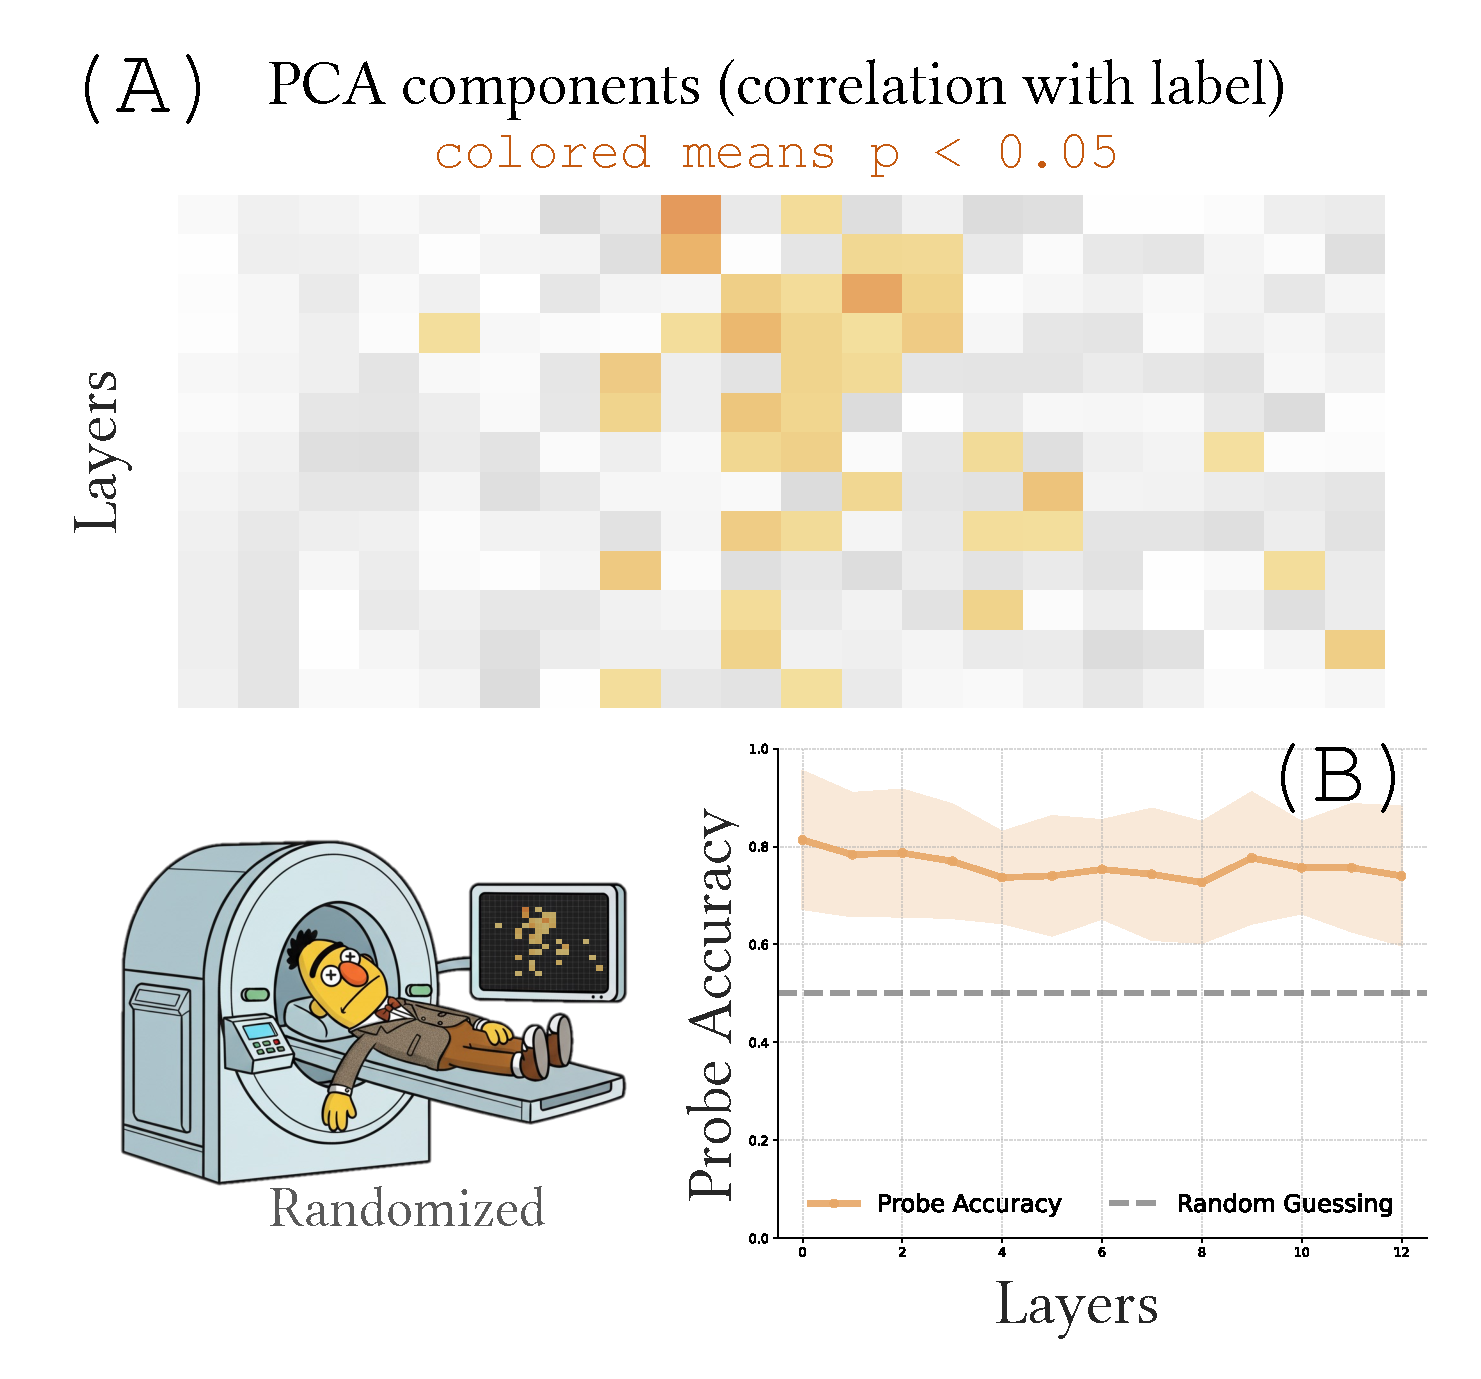
\includegraphics[width=\linewidth]{images/dead_bert.pdf}
    \caption{\textbf{Minimal dead salmon artifacts}. We extract token representations from a randomly initialized BERT for 300 IMDb sentences and average over sequence length. (A) Several principal components are spuriously correlated with sentiment labels. (B) A simple probe trained on layer representations achieves nontrivial cross-validated accuracy.}
    \label{fig:illus}
    \vspace{-2em}
\end{wrapfigure}

Beyond neuroscience and AI, such challenges are not unprecedented. Psychology and the social sciences faced a similar reckoning during the replication crisis, when questionable research practices produced widespread false positives \citep{doi:10.1126/science.aac4716,simmons2011false,ioannidis2005most,schimmack2020meta}. These fields responded with methodological reforms: pre-registration, registered reports, increased statistical power, and explicit multiple-comparison corrections \citep{munafo2017manifesto,korbmacher2023replication}. Likewise, econometrics used causal inference~\citep{pearl_causality} to formalize the distinction between correlation and causation, developing identification criteria, sensitivity analyses, and robustness tests \citep{imbens2015causal,angrist2009mostly,heckman2007economics}.

Now, AI interpretability can also begin to build its own methodological guardrails. As argued before, this requires both technical innovation and philosophical clarity \citep{miller2019explanation,williams2025mechanisticinterpretabilityneedsphilosophy}. This means clarifying our epistemic goals by answering: what does it mean to ``explain'' a neural network? \citep{lillicrap2019doesmeanunderstandneural,lipton2018mythos} Mechanistic interpretability embodies a type of \textit{scientific realism}, aiming to discover the \textit{one true} explanatory algorithm~\citep{psillos2005scientific,chakravartty2011scientific}. However, there is a significant push-back against the feasibility of this research project~\citep{rudin2019stop,P_ez_2019,saphra2024mechanistic}, motivating a shift toward pragmatic approaches prioritizing the utility of the explanations for specific downstream goals~\citep{zou2025representationengineeringtopdownapproach}. Here, we align with the pragmatic stance~\citep{Dewey1948-DEWRIP,chang2004inventing,potochnik2017idealization}, where explanations are seen as useful models that enable prediction, manipulation, and control~\citep{van1980scientific,cartwright1983laws}. 

\textbf{This work.} We analyze failure modes of contemporary AI interpretability methods, ranging from striking dead-salmon false positives to broader forms of statistical fragility, including poor generalization and high variance. We argue that these pathologies share a common root cause: the non-identifiability of many interpretability queries, compounded by the lack of principled uncertainty quantification, where non-identifiability manifests as high-variance estimates that should be reflected in large uncertainty. Diagnosing and addressing these issues, as well as articulating a coherent pragmatic research direction for interpretability, requires reframing AI interpretability as a problem of statistical (causal) inference. Accordingly, we propose one such statistical–causal reframing in which explanations are treated as parameters inferred from computational traces, enabling uncertainty-aware evaluation against meaningful alternative computational hypotheses.


% In 2009, researchers placed a dead salmon in an MRI scanner, showed it photographs of humans in social situations, and ostensibly asked it to judge their emotions \citep{bennett2009neural}. Standard analysis pipelines commonly used at the time surprisingly returned brain voxels as significantly predictive of emotional situations. The error arose from a failure to correct for multiple comparisons within the statistical analysis pipeline. 

% AI interpretability now faces its own \textit{dead salmon} issues. A growing body of work has shown that many influential methods, including feature attribution \citep{adebayo2018sanity}, probing classifiers \citep{ravichander-etal-2021-probing}, sparse autoencoders \citep{heap2025sparseautoencodersinterpretrandomly}, circuit discoveries \citep{melouxeverything}, and causal abstractions~\citep{sutter2025nonlinearrepresentationdilemmacausal}, can yield plausible-looking explanations even when applied to \textbf{random neural networks}. In Figure~\ref{fig:illus}, we report a minimum dead salmon artifact from analyzing activations of randomized BERT model in a sentiment analysis task where both correlation analysis and probing find highly significant \textit{explanations}. Yet, as modern AI systems are increasingly deployed in high-stake domains, AI interpretability becomes essential for transparency, accountability, and error diagnosis~\citep{mehrabi2021survey,barnes2024navigating,ramachandram2025transparentaicaseinterpretability}. Regulators have taken note: under both the GDPR and the EU AI Act, explainability is now a legal requirement~\citep{lore2023ai,Fresz_2024,kiseleva2022transparency,bengio2024international}.
% Interpretability methods could surface critical failure modes~\citep{kim2017interpretable,zech2018variable,caruana2015intelligible,meng2022locating,monea2024glitchmatrixlocatingdetecting,nguyen2025deploying} and offer levers for mitigating bias and systematic errors \citep{arrieta2019explainableartificialintelligencexai,kristofik2025bias,lepori-etal-2025-racing}. 

% A closely related methodological reckoning occurred in cognitive neuroscience during the rapid expansion of fMRI research. Following the “dead salmon” demonstration of false positives, an influential study showed that different research groups obtained divergent results even when they were given the same dataset and research question  \citep{botvinik2020variability}. 
% Subsequent work identified several sources of fragility. Widely used statistical procedures embedded in standard analysis pipelines were shown to inflate false-positive rates~\citep{eklund2016cluster}, an effect amplified by non-independent analyses producing spuriously large brain–behavior correlations~\citep{vul2009voodoo}. In addition, early neuroimaging research was constrained by small samples and limited data availability~\citep{button2013power,marek2022reproducible}, exacerbating overfitting, analytic flexibility, and spurious associations. Moreover, fMRI had been criticised for offering a small explanation on how the brain works - as opposed to its functional anatomy- resulting in little clinical relevances~\citep{lyon2017dead}. Finally, reverse inference emerged as a central interpretative problem, given that individual neural systems are not uniquely associated with specific cognitive functions~\citep{poldrack2006can,duncan2000common}. While data scarcity is less central in modern AI, the risks posed by misleading statistical signals and fragile interpretability directly carry over.
% % Also, interpretability should support communication and trust: non-experts are more willing to accept, contest, or regulate AI systems when their behavior can be faithfully explained~\citep{poursabzi2021manipulating,buccinca2021trust,organisation2023artificial}.


% %


% Despite frequent analogies to the \textit{neuroscience}~\citep{barrett2019analyzing}, \textit{biology}~\citep{lindsey2025biology} or \textit{physics} \citep{AL2023-cfg,AllenZhu-icml2024-tutorial} of neural networks, the practice of AI interpretability remains immature. Striking dead-salmon artifacts are accompanied by a general statistical fragility: small perturbations to inputs \citep{Ghorbani_Abid_Zou_2019,Kindermans2019,pmlr-v260-zhang25a} or changes in random initialization \citep{adebayo2018sanity,zafar-etal-2021-lack} can radically change explanations. Explanations often fail to generalize to new settings and input distributions \citep{hoelscherobermaier2023detectingeditfailureslarge}. Also, multiple incompatible explanations can be \textit{discovered} for the same behavior~\citep{melouxeverything,NEURIPS2019_bb836c01}. While the dead salmon study demonstrated a simple statistical oversight correctable through multiple comparison adjustments, AI interpretability's susceptibility to false discoveries stems from a more fundamental issue: the computational traces available do not uniquely determine explanations within typical hypothesis classes.



% Such challenges are not unprecedented. Psychology and the social sciences faced a similar reckoning during the replication crisis, when questionable research practices produced widespread false positives \citep{doi:10.1126/science.aac4716,simmons2011false,ioannidis2005most,schimmack2020meta}. These fields responded with methodological reforms: pre-registration, registered reports, increased statistical power, and explicit multiple-comparison corrections \citep{munafo2017manifesto,korbmacher2023replication}. Likewise, econometrics used causal inference~\citep{pearl_causality} to formalize the distinction between correlation and causation, developing identification criteria, sensitivity analyses, and robustness tests \citep{imbens2015causal,angrist2009mostly,heckman2007economics}.

% AI interpretability can also begin to build its own methodological guardrails. As argued elsewhere, this requires both technical innovation and philosophical clarity \citep{miller2019explanation,williams2025mechanisticinterpretabilityneedsphilosophy}. We will have to clarify our epistemic goals answering: what does it mean to ``explain'' a neural network? \citep{lillicrap2019doesmeanunderstandneural,lipton2018mythos} Mechanistic interpretability embodies a type of \textit{scientific realism}, aiming to discover the \textit{one true} mind-independent explanatory algorithm~\citep{psillos2005scientific,chakravartty2011scientific}. However, there is a significant pushback against the feasability of the realist stance~\citep{rudin2019stop,P_ez_2019,saphra2024mechanistic} motivating a shift toward pragmatic approaches prioritizing the utility of the explanations~\citep{zou2025representationengineeringtopdownapproach}.
% AI interpretability can draw concrete inspiration and build its own methodological guardrails. As argued elsewhere, this will require both technical innovation and philosophical clarity \citep{miller2019explanation,williams2025mechanisticinterpretabilityneedsphilosophy}. We will have to clarify our epistemic goals answering the question: what does it mean to ``explain'' a neural network? \citep{lillicrap2019doesmeanunderstandneural,lipton2018mythos}

% One approach to post hoc explanation is rooted in the philosophical framework of \textit{scientific realism}, which assumes that successful scientific theories approximately describe mind-independent reality~\citep{psillos2005scientific,chakravartty2011scientific}. Typically, mechanistic interpretability embodies this perspective~\citep{olah2020zoom,elhage2021mathematical}. However, there is a pushback against the realist stance~\citep{rudin2019stop,P_ez_2019,saphra2024mechanistic} motivating a shift toward pragmatic approaches prioritizing utility of the explanations~\cite{zou2025representationengineeringtopdownapproach}.

% \paragraph{This work.}
% Our analysis of failures further supports a pragmatist perspective on AI explanations. We argue that their root cause lies in a general problem of \textbf{non-identifiability}: computational traces do not uniquely determine an explanation within the assumed hypothesis classes. However, identifiability is a statistical notion; understanding and addressing it requires framing interpretability as a problem of statistical-causal inference. 

% We outline one such possible formalism by treating explanations as \emph{structured objects} (surrogate models) to be inferred from computational traces. This framework enforces the explicit and precise statement of \textit{what should be explained (including the generalization scope)} and \textit{what counts as an explanation}. The framework does not prescribe what researchers ought to study, it simply lays out the agenda of framing such choices within the rigorous framework of statistical-causal inference. Then, interpretability methods become \textbf{estimators} producing an estimated explanation (e.g., maximum likelihood explanation from the postulated hypothesis class) from computational traces with proper uncertainty quantification. The identifiability of an interpretability task can then be studied formally using the existing tools of statistical-causal inference. This brings to bear all the toolkit of statistical inference, which we demonstrate with hypothesis testing as a simple and immediate tool to eliminate all dead salmon artifacts, even within non-identifiable interpretability tasks. 

% Overall, this perspective aligns with the pragmatist stance~\citep{P_ez_2019, Dewey1948-DEWRIP,chang2004inventing,potochnik2017idealization}, where explanations are useful models that enable prediction, manipulation, and control~\citep{van1980scientific,cartwright1983laws}.

% Our analysis of interpretability failures further supports a pragmatist perspective on AI explanations. We argue that their root cause lies in a general problem of \textbf{non-identifiability}: computational traces do not uniquely determine an explanation within the assumed hypothesis classes. Identifiability is a statistical notion; understanding and addressing it requires framing interpretability as a problem of statistical-causal inference. 

% We outline one such possible formalism by treating explanations as \emph{structured objects} (surrogate models) to be inferred from computational traces. This framework enforces the explicit and precise statement of \textit{what should be explained (including the generalization scope)} and \textit{what counts as an explanation}, the pragmatic error measurement quantifying how well a candidate explanation fits the computational traces. This does not prescribe what researchers ought to study, it lays out the agenda of framing such choices within the rigorous framework of statistical-causal inference. Then, interpretability methods become estimators producing an estimated explanation from computational traces with proper uncertainty quantification.  Questions about the identifiability of an interpretability task can be studied formally using the existing tools of statistical-causal inference. This brings to bear all the toolkit of statistical inference, which we demonstrate with hypothesis testing as a simple and immediate tool to eliminate all dead salmon artifacts, even within non-identifiable interpretability tasks.
% % 
% This perspective aligns with the pragmatist stance~\citep{P_ez_2019, Dewey1948-DEWRIP,chang2004inventing,potochnik2017idealization}, explanations are useful models that enable prediction, manipulation, and control~\citep{van1980scientific,cartwright1983laws}. 

% This reframing sidesteps intractable debates about the \textit{true mechanisms} encoded in neural networks, focusing instead on whether proposed explanations fulfill their intended purposes~\citep{van1980scientific,cartwright1983laws,potochnik2017idealization}.

% This work and the tentative formalization do not prescribe which queries or hypothesis spaces researchers ought to study, it lays out the agenda of clearly stating these assumptions to study. Once specified, they can be examined using the full toolkit of statistical inference, enabling transparent comparison between methods, theoretical analysis of their assumptions, and ultimately, the design of scientifically grounded interpretability approaches with proper uncertainty estimation.

% Our analysis of interpretability failures further supports a pragmatist perspective on AI explanations. We argue that the root cause is a general problem of \textbf{non-identifiability}: the observable computational traces do not uniquely determine an explanation within the postulated hypothesis class. Because interpretability has yet to be formalized as a problem of statistical inference, identifiability is currently just a metaphor. Without the tool to properly study it, we only observe the manifestations of non-identifiable explanatory goals: lack of generalization, multiple incompatible explanations, sensitivity to design choices, and striking false discoveries such as dead salmon artifacts.

% We sketch a statistical--causal reframing of interpretability tasks, where explanations are treated as \emph{surrogate models} answering a specified set of (causal) queries about a target model’s behavior. The framework requires three explicit components: (i) the queries to be answered (\textit{what should be explained}); (ii) the hypothesis space of admissible explanations, e.g., circuits, probes, algorithmic descriptions (\textit{what counts as an explanation}); and (iii) an error measure to quantify how well a candidate explanation answers the queries. This views interpretabilty as an inference protocol that should quantify uncertainty, controls error rates, and incorporates robustness checks, such as randomized-network baselines. Interpretability methods become formal estimators whose statistical properties such as variance, or consistency can be rigorously studied. Furthermore, identifiability properties become a critical question about the interpretability tasks.

% This perspective aligns with, and operationalizes, the pragmatist stance~\cite{P_ez_2019}. Following Dewey’s instrumentalism \citep{Dewey1948-DEWRIP}, as well as subsequent pragmatist philosophers of science \citep{chang2004inventing,potochnik2017idealization}, explanations are useful models enabling prediction and intervention for questions of interest. This sidesteps intractable debates about the \textit{true mechanisms} embedded within neural networks, focusing instead on whether proposed explanations serve their intended purposes~\citep{van1980scientific,cartwright1983laws,potochnik2017idealization}. 

% Crucially, the statistical--causal framing does not prescribe which queries or hypothesis spaces \textit{should be} studied; rather, it requires that these choices be made explicit. This transparency enables rigorous comparison, theoretical analysis (e.g., identifiability), and ultimately the development of concrete, scientifically grounded interpretability approaches using the well-established tools of statistical and causal inference.

% Echoing Van Fraassen’s notion of \textit{constructive empiricism}~\citep{van1980scientific}, Cartwright’s \textit{useful fictions}~\citep{cartwright1983laws}, and Potochnik’s \textit{idealization framework}~\citep{potochnik2017idealization}, we treat interpretability as the design of computationally adequate models that trade completeness for applicability in a causally complex world.



% In 2012, the Ig Nobel Prize for neuroscience was awarded to a surprising result: researchers placed a dead salmon in an fMRI scanner, showed it photographs of humans, and ostensibly \textit{asked} it to judge their emotions \citep{bennett2009neural}. Standard pipelines identified several brain regions as predictive. The explanation, of course, was not supernatural cognition but a failure to correct for multiple comparisons: random noise produced apparently meaningful signals.

% Now, AI interpretability faces its own dead salmons. Many methods including feature attribution \citep{adebayo2018sanity}, probing classifiers \citep{ravichander-etal-2021-probing}, sparse autoencoders \citep{heap2025sparseautoencodersinterpretrandomly}, circuit discovery \citep{melouxeverything}, and causal abstraction~\citep{sutter2025nonlinearrepresentationdilemmacausal} have been shown to produce plausible-looking explanations within random neural networks. Beyond these striking false positives, interpretability methods also display statistical fragility. Small perturbations to the input \citep{Ghorbani_Abid_Zou_2019,Kindermans2019,pmlr-v260-zhang25a} or changes in random initialization \citep{adebayo2018sanity,zafar-etal-2021-lack} can drastically change the explanations. In mechanistic interpretability, interventions on identified circuits often fail to generalize: edits that succeed in one context may break in another \citep{hoelscherobermaier2023detectingeditfailureslarge}. Conversely, multiple incompatible explanations can be found for the exact same behavior~\citep{melouxeverything,NEURIPS2019_bb836c01}. These problems are not isolated failures of simple misapplied uncertainty estimation but symptoms of a deeper methodological gap: interpretability research currently lacks the statistical and causal foundations that characterize mature empirical sciences.

% Yet, the stakes are high. AI systems are increasingly deployed in real-world settings, where their decisions directly affect human lives. In such contexts, interpretability is essential for transparency, accountability, and error diagnosis \citep{mehrabi2021survey,barnes2024navigating,ramachandram2025transparentaicaseinterpretability}. Regulators have recognized these risks: under both the GDPR and the EU AI Act, explainability is now a legal requirement\footnote{Regulation (EU) 2016/679, \url{https://eur-lex.europa.eu/eli/reg/2016/679/oj}; Regulation (EU) 2024/1689, \url{https://eur-lex.europa.eu/eli/reg/2024/1689/oj/eng}} \citep{lore2023ai,Fresz_2024,kiseleva2022transparency,bengio2024international}. 
% % 
% Interpretability methods could uncovered critical failure modes in safety-sensitive domains such as autonomous driving \citep{kim2017interpretable}, medical decision support \citep{zech2018variable,caruana2015intelligible}, and large language models \citep{meng2022locating,monea2024glitchmatrixlocatingdetecting}. They promise levers for mitigating bias and correcting errors \citep{arrieta2019explainableartificialintelligencexai,kristofik2025bias}, and they aim to enable human--AI collaboration, where operators can meaningfully supervise, understand, and override automated decisions when needed \citep{felzmann2020towards,kim2018interpretability}. At the societal level, interpretability should supports communication and trust: non-experts are more willing to accept, contest, or regulate AI systems when their behavior can be faithfully explained \citep{poursabzi2021manipulating,buccinca2021trust,organisation2023artificial}.


% AI interpretability has often been framed metaphorically as the \textit{biology}~\citep{lindsey2025biology} or \textit{physics}~\citep{AL2023-cfg,AllenZhu-icml2024-tutorial} of LLMs, where the AI systems become the objects of study. Despite this ambition, a proper scientific practice of AI interpretability is still lacking, as revealed by the recurring problems of underspecification, instability, lack of generalization, and false discoveries. 
% % 
% Such problems are not unique to AI interpretability, they echo past crises faced by other empirical sciences. In psychology and social sciences, the \textit{replication crisis} exposed how questionable research practices (p-hacking, selective reporting, HARKing) led to widespread false positives, with landmark studies failing to replicate at alarmingly high rates \citep{doi:10.1126/science.aac4716,simmons2011false,ioannidis2005most,schimmack2020meta}. These fields responded with methodological reforms: pre-registration, registered reports, increased statistical power, and explicit multiple comparison corrections \citep{munafo2017manifesto,korbmacher2023replication}. 
% % 
% Similarly, econometrics and causal inference have developed rigorous frameworks to distinguish correlation from causation~\citep{pearl_causality}, addressing problems of confounding, selection bias, and model misspecification through methods like instrumental variables, difference-in-differences, and regression discontinuity designs \citep{imbens2015causal,angrist2009mostly,heckman2007economics}. These fields have established formal criteria for identification, developed sensitivity analyses for untestable assumptions, and emphasized the importance of specification tests and robustness checks. AI interpretability can draw concrete inspiration from these mature methodologies.


% As argued before, addressing the issues of AI interpretability will require both technical innovation and philosophical clarity \citep{miller2019explanation,williams2025mechanisticinterpretabilityneedsphilosophy}. We must first confront a fundamental question: What does it mean to ``explain'' a neural network? \citep{lillicrap2019doesmeanunderstandneural}
% % 
% One approach to post-hoc explanation is rooted in the philosophical framework of \textit{scientific realism}, which assumes that successful scientific theories approximately describe mind-independent reality and that scientific progress consists in getting closer to \textit{the truth} about the world's underlying structure \citep{psillos2005scientific,chakravartty2011scientific}. Applied to interpretability, this view suggests we seek to discover how networks ``truly'' work—to uncover their real mechanisms. Some work in mechanistic interpretability explicitly or implicitly embodies this perspective, searching for the "true" circuits or features that constitute the network's computational architecture \citep{olah2020zoom,elhage2021mathematical}.

% However, there is pushback against this realist stance~\citep{saphra2024mechanistic}. \citet{rudin2019stop} argues that we should in fact abandon efforts to explain black-box models in high-stakes settings and instead build inherently interpretable models from the start, noting that post-hoc explanations ``must be wrong'' since perfect fidelity would make the explanation equivalent to the original model. \citet{lipton2018mythos} exposes ambiguities in what ``interpretability'' even means, showing that the concept is underspecified and that different stakeholders have incompatible notions of what makes a model interpretable. 
% % 
% This skepticism has motivated a shift toward more pragmatic approaches that prioritize utility over truth. Representation engineering (RepE) \citep{zou2025representationengineeringtopdownapproach} exemplifies this instrumentalist stance: rather than seeking to reverse-engineer networks into interpretable source code, RepE identifies high-level representations (honesty, harmfulness, sentiment) that can be read out or manipulated to control model behavior, treating these representations as useful abstractions rather than claims about the network's "true" internal structure \citep{zou2025representationengineeringtopdownapproach,turner2024steeringlanguagemodelsactivation}. This top-down approach abstracts away low-level mechanistic details, focusing instead on whether interventions reliably produce desired outcomes—a perspective aligned with pragmatist and instrumentalist philosophies of science.

% In this work, we embrace and aim to further advance the \emph{pragmatist stance}, following philosophers of science from Dewey's instrumentalism \citep{dewey1920reconstruction,dewey1925experience} to \citet{chang2004inventing} and \citet{potochnik2017idealization}: explanations are not discoveries of pre-existing truth but \emph{useful models} that enable prediction and intervention for the type of questions we are interested in. This sidesteps intractable debates about whether networks have ``real'' mechanisms, focusing instead on whether proposed explanations serve their intended purposes. As \citet{van1980scientific} argues for ``constructive empiricism,'' we seek computationally adequate models rather than true representations. Similarly, \citet{cartwright1983laws} shows that scientific models are ``useful fictions'' that trade completeness for applicability, and \citet{potochnik2017idealization} demonstrates that idealization is not a bug but a feature of science—that all scientific understanding necessarily involves simplification and that the value of a model lies in its ability to support human cognitive and practical ends in a complex world.

% Crucially, this pragmatic stance is compatible with—indeed, demands—rigorous statistical inference. By explicitly specifying explanatory aims (which questions must the explanation answer? and what does the explanation should look like?), we can rigorously test explanation quality, quantify uncertainty, and guard against false discoveries. The key is \emph{operationalization}: making precise what counts as a good explanation for a given interpretability task \citep{tal2015measurement,chang2004inventing}. This approach resolves apparent contradictions: we can use "false" idealized models \citep{potochnik2017idealization} while maintaining scientific rigor, because the models' value derives not from literal truth but from their capacity to answer specific questions reliably.


% \textbf{In this work}, we first document that major interpretability paradigms—attribution, probing, concept discovery, circuit analysis—all exhibit systematic vulnerabilities to false positives, with dead salmon artifacts (explaining random networks) as the most striking manifestation. Then, to embrace the instrumentalist perspective and make AI interpretability more rigorous, we propose one possible formalization of AI interpretability as a statistical-causal inference task, where explanations are surrogate models answering a specified set of (causal and statistical) queries. This makes identifiability, uncertainty, and hypothesis testing precise. 

% The main advantage of this formalization is that it forces the explicit statement of the explanatory aims (via the set of queries to be answered) and the explanation form (via the specification of hypothesis space of candidate explanations, e.g., circuit, algorithms, probe). It offers a way to bring in the whole toolkit of statistical-causal analysis to the world of AI interpretability, which offers endless theoretical and practical tools to progressively build a rigorous methodology. In this perspective, interpretability methods are estimators whose statistical properties such as variance, bias, and consistency become well-defined. 

% As a toy applicative example, we show how dead salmon issues can be easily fixed by using the hypothesis testing framework and comparing against a null hypothesis consisting of applying the interpretability method in randomized networks—a direct parallel to the multiple comparison corrections that resolved the original dead salmon problem in fMRI research. We outline a broader research agenda, including Bayesian interpretability, cross-validation for interpretability methods, and identifiability analysis for causal claims, drawing explicitly on the methodological innovations that helped psychology, econometrics, and other fields overcome their own replication crises.

